\documentclass[journal=jcim,manuscript=suppinfo]{achemso}
\usepackage{amsmath}
\usepackage{graphicx}
\usepackage{hyperref}
\usepackage[table,xcdraw]{xcolor}
\usepackage[left=1.5cm, right=1cm]{geometry}
\usepackage{multirow}
\usepackage{csvsimple}
\usepackage{rotating}
\usepackage{longtable}
\usepackage{tabularx}
\usepackage{booktabs}


\makeatletter
\let\oldminipage\minipage
\let\oldendminipage\endminipage
\renewenvironment{minipage}[1]{}{}
\g@addto@macro{\maketitle}{\let\minipage\oldminipage\let\endminipage\oldendminipage}
\makeatother


% fix some achemso rubbish
\renewcommand{\titlesize}{\normalsize}
\renewcommand{\affilsize}{\footnotesize	}
\renewcommand{\authorsize}{\footnotesize	}
\renewcommand{\emailsize}{\footnotesize}


%% Main manuscript contributors
\author{Hugo MacDermott-Opeskin}
\affiliation{Open Molecular Software Foundation, Davis CA, USA}
\author{Jenke Scheen}
\affiliation{Open Molecular Software Foundation, Davis CA, USA}
\author{Cas Wognum}
\affiliation{Valence Labs, Montréal, Québec, Canada}
\altaffiliation{Recursion Pharmaceuticals, Salt Lake City, UT, USA}
\author{Joshua, T Horton}
\affiliation{Open Molecular Software Foundation, Davis CA, USA}
\author{Devany West}
\affiliation{Open Molecular Software Foundation, Davis CA, USA}
\author{Alexander Matthew Payne}
\affiliation{Computational and Systems Biology Program, Memorial Sloan Kettering Cancer Center, New York, NY, USA}
\altaffiliation{Tri-Institutional PhD Program in Chemical Biology, Memorial Sloan Kettering Cancer Center, New York, NY, USA}
\author{Maria A Castellanos}
\affiliation{Computational and Systems Biology Program, Memorial Sloan Kettering Cancer Center, New York, NY, USA}
\author{Sean Colby}
\affiliation{Open Molecular Software Foundation, Davis CA, USA}

%% ASAP %%
\author{Edward Griffen}
\affiliation{MedChemica Consultancy Ltd, Macclesfield, UK}
\author{David Cousins}
\affiliation{MedChemica Consultancy Ltd, Macclesfield, UK}
\author{Jessica Stacey}
\affiliation{MedChemica Consultancy Ltd, Macclesfield, UK}
\author{Lauren Reid}
\affiliation{MedChemica Consultancy Ltd, Macclesfield, UK}
\author{Jasmin Cara Aschenbrenner}
\affiliation{Diamond Light Source, Didcot, UK}
\author{Daren Fearon}
\affiliation{Diamond Light Source, Didcot, UK}
\author{Blake Balcomb}
\affiliation{Diamond Light Source, Didcot, UK}
\author{Peter Marples}
\affiliation{Diamond Light Source, Didcot, UK}
\author{Charles W.E. Tomlinson}
\affiliation{Diamond Light Source, Didcot, UK}
\author{Ryan Lithgo}
\affiliation{Diamond Light Source, Didcot, UK}
\author{Max Winokan}
\affiliation{Diamond Light Source, Didcot, UK}
\author{Haim Barr}
\affiliation{Weizmann Institute of Science, Rehovot, IL}
\author{Noa Lahav}
\affiliation{Weizmann Institute of Science, Rehovot, IL}
\author{Michael Lavi}
\affiliation{Weizmann Institute of Science, Rehovot, IL}
\author{Shirley Duberstein}
\affiliation{Weizmann Institute of Science, Rehovot, IL}
\author{Galit Cohen}
\affiliation{Weizmann Institute of Science, Rehovot, IL}
\author{Gwendolyn Fate}
\affiliation{Thames Pharma Partners, USA}
\author{Bruce Lefker}
\affiliation{Thames Pharma Partners, USA}
\author{Ralph Robinson}
\affiliation{Thames Pharma Partners, USA}
\author{Tamas Szommer}
\affiliation{Centre for Medicines Discovery, Oxford, UK}
\author{Nick Lynch}
\affiliation{Curlew Research, UK}


%% OpenADMET
\author{Mallory Tollefson}
\affiliation{Open Molecular Software Foundation, Davis CA, USA}
\author{Cynthia Xu}
\affiliation{Open Molecular Software Foundation, Davis CA, USA}

% Valence 
\author{Jonny Hsu}
\affiliation{Valence Labs, Montréal, Québec, Canada}
\altaffiliation{Recursion Pharmaceuticals, Salt Lake City, UT, USA}
\author{Julien St-Laurent}
\affiliation{Valence Labs, Montréal, Québec, Canada}
\altaffiliation{Recursion Pharmaceuticals, Salt Lake City, UT, USA}
\author{Honore Etsmoberg}
\affiliation{Valence Labs, Montréal, Québec, Canada}
\altaffiliation{Recursion Pharmaceuticals, Salt Lake City, UT, USA}
\author{Lu Zhu}
\affiliation{Valence Labs, Montréal, Québec, Canada}
\altaffiliation{Recursion Pharmaceuticals, Salt Lake City, UT, USA}
\author{Andrew Quirke}
\affiliation{Valence Labs, Montréal, Québec, Canada}
\altaffiliation{Recursion Pharmaceuticals, Salt Lake City, UT, USA}
\author{Oscar Mendez-Lucio}
\affiliation{Recursion Pharmaceuticals, Salt Lake City, UT, USA}

%% Participants
% All participants excluding the authors already listed in the main document
\author{Mohamed Iliyas Abdul Haleem}
\affiliation{Independent Researcher}

\author{Irfan Alibay}
\affiliation{Open Molecular Software Foundation, Davis CA, USA}

\author{Gunjan Baid}
\affiliation{Inductive Bio, New York, NY, USA}

\author{Benjamin Birnbaum}
\affiliation{Inductive Bio, New York, NY, USA}

\author{Kevin P. Bishop}
\affiliation{Ontario Institute for Cancer Research, Toronto, ON, Canada}

\author{Laurent Hoffer}
\affiliation{Ontario Institute for Cancer Research, Toronto, ON, Canada}

\author{Hugo Bohorquez}
\affiliation{Ontario Institute for Cancer Research, Toronto, ON, Canada}

\author{Ashmita Bose}
\affiliation{University of Luxembourg, Luxembourg City, Luxembourg}

\author{C.J. Brown}
\affiliation{Alpha29, LLC}

\author{Jackson Burns}
\affiliation{MIT, Cambridge, MA, USA}

\author{Lianjin Cai}
\affiliation{University of Pittsburgh, Pittsburgh, PA, USA}

\author{Ruel Cedeno}
\affiliation{Novalix, 67000 Strasbourg, France}

\author{Vladimir Chupakhin}
\affiliation{Simulations Plus, Research Triangle Park, NC, USA}

\author{Finlay Clark}
\affiliation{Newcastle University, Newcastle, UK}

\author{Daniel J Cole}
\affiliation{School of Natural and Environmental Sciences, Newcastle University, Newcastle Upon Tyne, NE1 7RU, UK}

\author{Carles Corbi-Verge}
\affiliation{Recursion, Salt Lake City, UT, USA}

\author{Muhammad Danial}
\affiliation{Shenzhen Institute of Synthetic Biology, Shenzhen Institutes of Advanced Technology, Chinese Academy of Sciences, Shenzhen 518055, China}

\author{Alec Davi}
\affiliation{Owkin, New York, NY, USA}

\author{Wim Dehaen}
\affiliation{Department of Organic Chemistry, Faculty of Chemical Technology, University of Chemistry and Technology Prague, Technická 5, Prague 6 166 28, Czech Republic}
\altaffiliation{Department of Informatics and Chemistry, Faculty of Chemical Technology, University of Chemistry and Technology Prague,  Technická 5, Prague 6 166 28, Czech Republic}

\author{Niklas Piet Doering}
\affiliation{Freie Universität Berlin, Berlin, Germany}

\author{Gerhard Wolber}
\affiliation{Freie Universität Berlin, Berlin, Germany}

\author{Alexis Dougha}
\affiliation{BFA, Université Paris Cité, CNRS UMR 8251, Inserm U1133, 75013 Paris, France}

\author{Bryce Eakin}
\affiliation{Inductive Bio, New York, NY, USA}

\author{Anatol Ehrlich}
\affiliation{University of Vienna, Vienna, Austria}

\author{Rokas Elijosius} % [Pending check]
\affiliation{University of Cambridge, Cambridge, UK}

\author{Jozef Fülöp}
\affiliation{Department of Informatics and Chemistry, Faculty of Chemical Technology, University of Chemistry and Technology Prague, Technická 5, Prague 6 166 28, Czech Republic}

\author{Anthony Gitter}
\affiliation{University of Wisconsin-Madison, Madison, WI, USA}
\altaffiliation{Morgridge Institute for Research, Madison, WI, USA}

\author{Yaowen Gu}
\affiliation{New York University, New York, NY, USA}

\author{Teresa Head-Gordon}
\affiliation{University of California, Berkeley, CA, USA}

\author{Ellena Jiang}
\affiliation{University of Vienna, Vienna, Austria}

\author{Benjamin Kaminow}
\affiliation{Computational and Systems Biology Program, Memorial Sloan Kettering Cancer Center, New York, NY, USA}

\author{Sina Khosravi}
\affiliation{Mashhad University of Medical Sciences, Mashhad, Khorasan Razavi, Iran}

\author{Asma Feriel Khoualdi} % [Pending check]
\affiliation{Newcastle University, Newcastle, UK}

\author{Eelke Bart Lenselink}
\affiliation{Galapagos NV, 2800 Mechelen, Belgium}

\author{Kenneth Goossens}
\affiliation{Galapagos NV, 2800 Mechelen, Belgium}


\author{Giovanni Tricarico}
\affiliation{Galapagos NV, 2800 Mechelen, Belgium}


\author{Johan Hofmans}
\affiliation{Galapagos NV, 2800 Mechelen, Belgium}

\author{Marie-Pierre Dréanic}
\affiliation{Galapagos NV, 2800 Mechelen, Belgium}

\author{Stephane de Cesco}
\affiliation{Galapagos NV, 2800 Mechelen, Belgium}

\author{Zhirong Liu}
\affiliation{Peking University, Beijing, China}

\author{Yue Liu}
\affiliation{University of Pittsburgh, Pittsburgh, PA, USA}

\author{Sijie Liu}
\affiliation{Freie Universität Berlin, Berlin, Germany}

\author{Yizhou Ma}
\affiliation{QuantaBricks, Newark, NJ, USA}

\author{Patrick Maher}
\affiliation{Inductive Bio, New York, NY, USA}

\author{Imke Mayer} % [Pending Check]
\affiliation{Owkin, New York, NY, USA}

\author{Antonia Mey}
\affiliation{University of Edinburgh, Edinburgh, Scotland, UK}

\author{Julien Michel}
\affiliation{University of Edinburgh, Edinburgh, Scotland, UK}


\author{Floriane Montanari} % [Pending check]
\affiliation{Owkin, New York, NY, USA}

\author{Taoyu Niu}
\affiliation{University of Pittsburgh, Pittsburgh, PA, USA}

\author{Ryusei Ogino}
\affiliation{Japan Tobacco INC., Minato City, Tokyo, Japan}

\author{Ashok Palaniappan}
\affiliation{SASTRA Deemed University, Thanjavur, Tamil Nadu 613401, India}

\author{Ida Titus}
\affiliation{SASTRA Deemed University, Thanjavur, Tamil Nadu 613401, India}

\author{Mounika Srilakshmi}
\affiliation{SASTRA Deemed University, Thanjavur, Tamil Nadu 613401, India}

\author{Xiaolin Pan}
\affiliation{New York University, New York, NY, USA}

\author{Auro Patnaik}
\affiliation{University of Edinburgh, Edinburgh, Scotland, UK}

\author{Long-Hung Pham}
\affiliation{Imperial College London, London, UK}

\author{Luis Pinto}
\affiliation{Independent Researcher}

\author{Justin Purnomo}
\affiliation{University of California, Berkeley, CA, USA}

\author{Alexander Rich}
\affiliation{Inductive Bio, New York, NY, USA}

\author{Lars Schaaf}
\affiliation{University of Cambridge, Cambridge, UK}

\author{Christoph Schran}
\affiliation{University of Cambridge, Cambridge, UK}

\author{Satya Pratik Srivastava}
\affiliation{Shiv Nadar University, Delhi NCR, India}

\author{Rajeev Kumar Singh}
\affiliation{Shiv Nadar University, Greater Noida, Uttar Pradesh, India}

\author{Kunyang Sun}
\affiliation{University of California, Berkeley, CA, USA}

\author{Zhaoxi Sun}
\affiliation{Shenzhen University of Advanced Technology, Shenzhen, China}

\author{Valerij Talagayev}
\affiliation{Freie Universität Berlin, Berlin, Germany}

\author{Balamurugan Thirukonda Subramanian Balakrishnan}
\affiliation{Independent Researcher}

\author{Alexandre Tkatchenko}
\affiliation{University of Luxembourg, Luxembourg City, Luxembourg}

\author{Wojtek Treyde}
\affiliation{University of Oxford, Oxford, UK}

\author{Austin Tripp}
\affiliation{Valence Labs, Quebec, Canada}

\author{Nopsinth Vithayapalert}
\affiliation{VISTEC, Pa Yup Nai, Thailand}

\author{Yingze Wang}
\affiliation{University of California, Berkeley, CA, USA}

\author{Azmine Toushik Wasi}
\affiliation{Shahjalal University of Science and Technology, Sylhet, Bangladesh}

\author{Steffen Wedig}
\affiliation{University of Cambridge, Cambridge, UK}

\author{Bofei Xu}
\affiliation{Peking University, Beijing, China}

\author{Weijun Zhou}
\affiliation{New York University, New York, NY, USA}



%% ASAP PIs
\author{Frank von Delft}
\affiliation{Diamond Light Source, Didcot, UK}
\author{Alpha Lee}
\affiliation{PostEra, Cambridge, MA, USA}
\author{Karla Kirkegaard}
\affiliation{Stanford University School of Medicine: Stanford, CA, US}
\author{Peter Sjö}
\affiliation{Drugs for Neglected Diseases initiative: Geneva, Genève, CH}

%% OpenADMET PIs
% \author{Sri Kosuri} 
% \affiliation{Octant Inc: Emeryville, CA, US}

\author{James S. Fraser}
\affiliation{University of California San Francisco, San Francisco, CA, USA}

%% John as final as PI across both
\author{John D. Chodera}
\affiliation{Computational and Systems Biology Program, Memorial Sloan Kettering Cancer Center, New York, NY, USA}

\email{*jenke.scheen@omsf.io}


% Title 
\title{A Computational Community Blind Challenge on Pan-Coronavirus Drug Discovery Data}

\begin{document}

\maketitle


\begin{figure}
    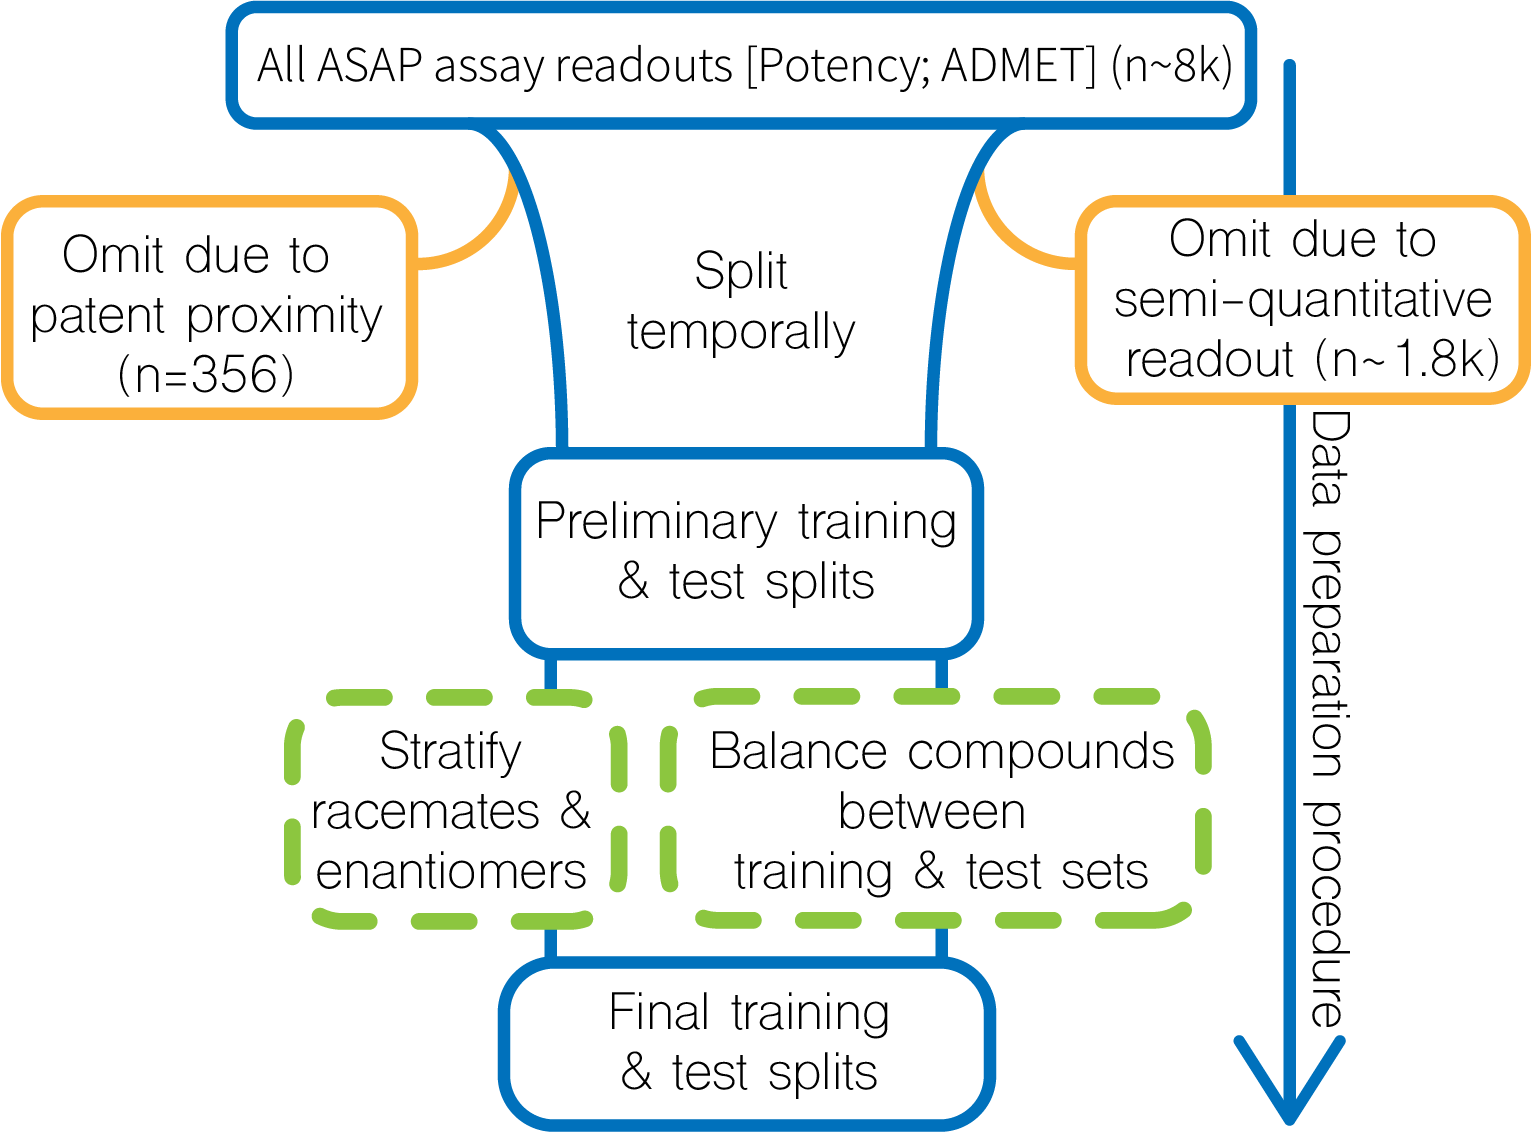
\includegraphics[scale=0.75]{SI/fig_S1_data_preparation/Figure.png}
  \caption{Data preparation workflow for the blind challenge. From $\sim$8k experimental measurements (top), 356 compound measurements were omitted completely from the challenge due to their proximity to the to-be-announced preclinical candidate. Another $\sim$1.8k measurements were removed due to their semi-quantitative nature (i.e. falling outside of assays' dynamic ranges). Remaining data was split temporally by synthesis actioning date at a 75/25 split. Finally, post-hoc adjustments were made to ensure that racemic/enantiomeric measurements were binned into same (training or test) set and that as many compounds as possible were assigned to the (training or test) set across subchallenges or ADMET endpoints.}
  \label{fgr:success_rate_lead_vs_backup}
\end{figure}



\begin{figure}
    
\includegraphics[scale=0.175]{SI/fig_S2_ADMET_dynamic_ranges/admet_endpoints.png}
    
\includegraphics[scale=0.175]{SI/fig_S2_ADMET_dynamic_ranges/admet_endpoints_log10.png}
  \caption{Distributions of ADMET endpoints for train (blue) and test (orange) show outlier and dynamic range difficulties.  HLM, MLM, and Permeability have long tails, KSOL, has mostly low and high values within this dynamic range.  Raw values (top) and log10 values (bottom).}
  \label{fgr:admet_endpoints}
\end{figure}



\begin{figure}
    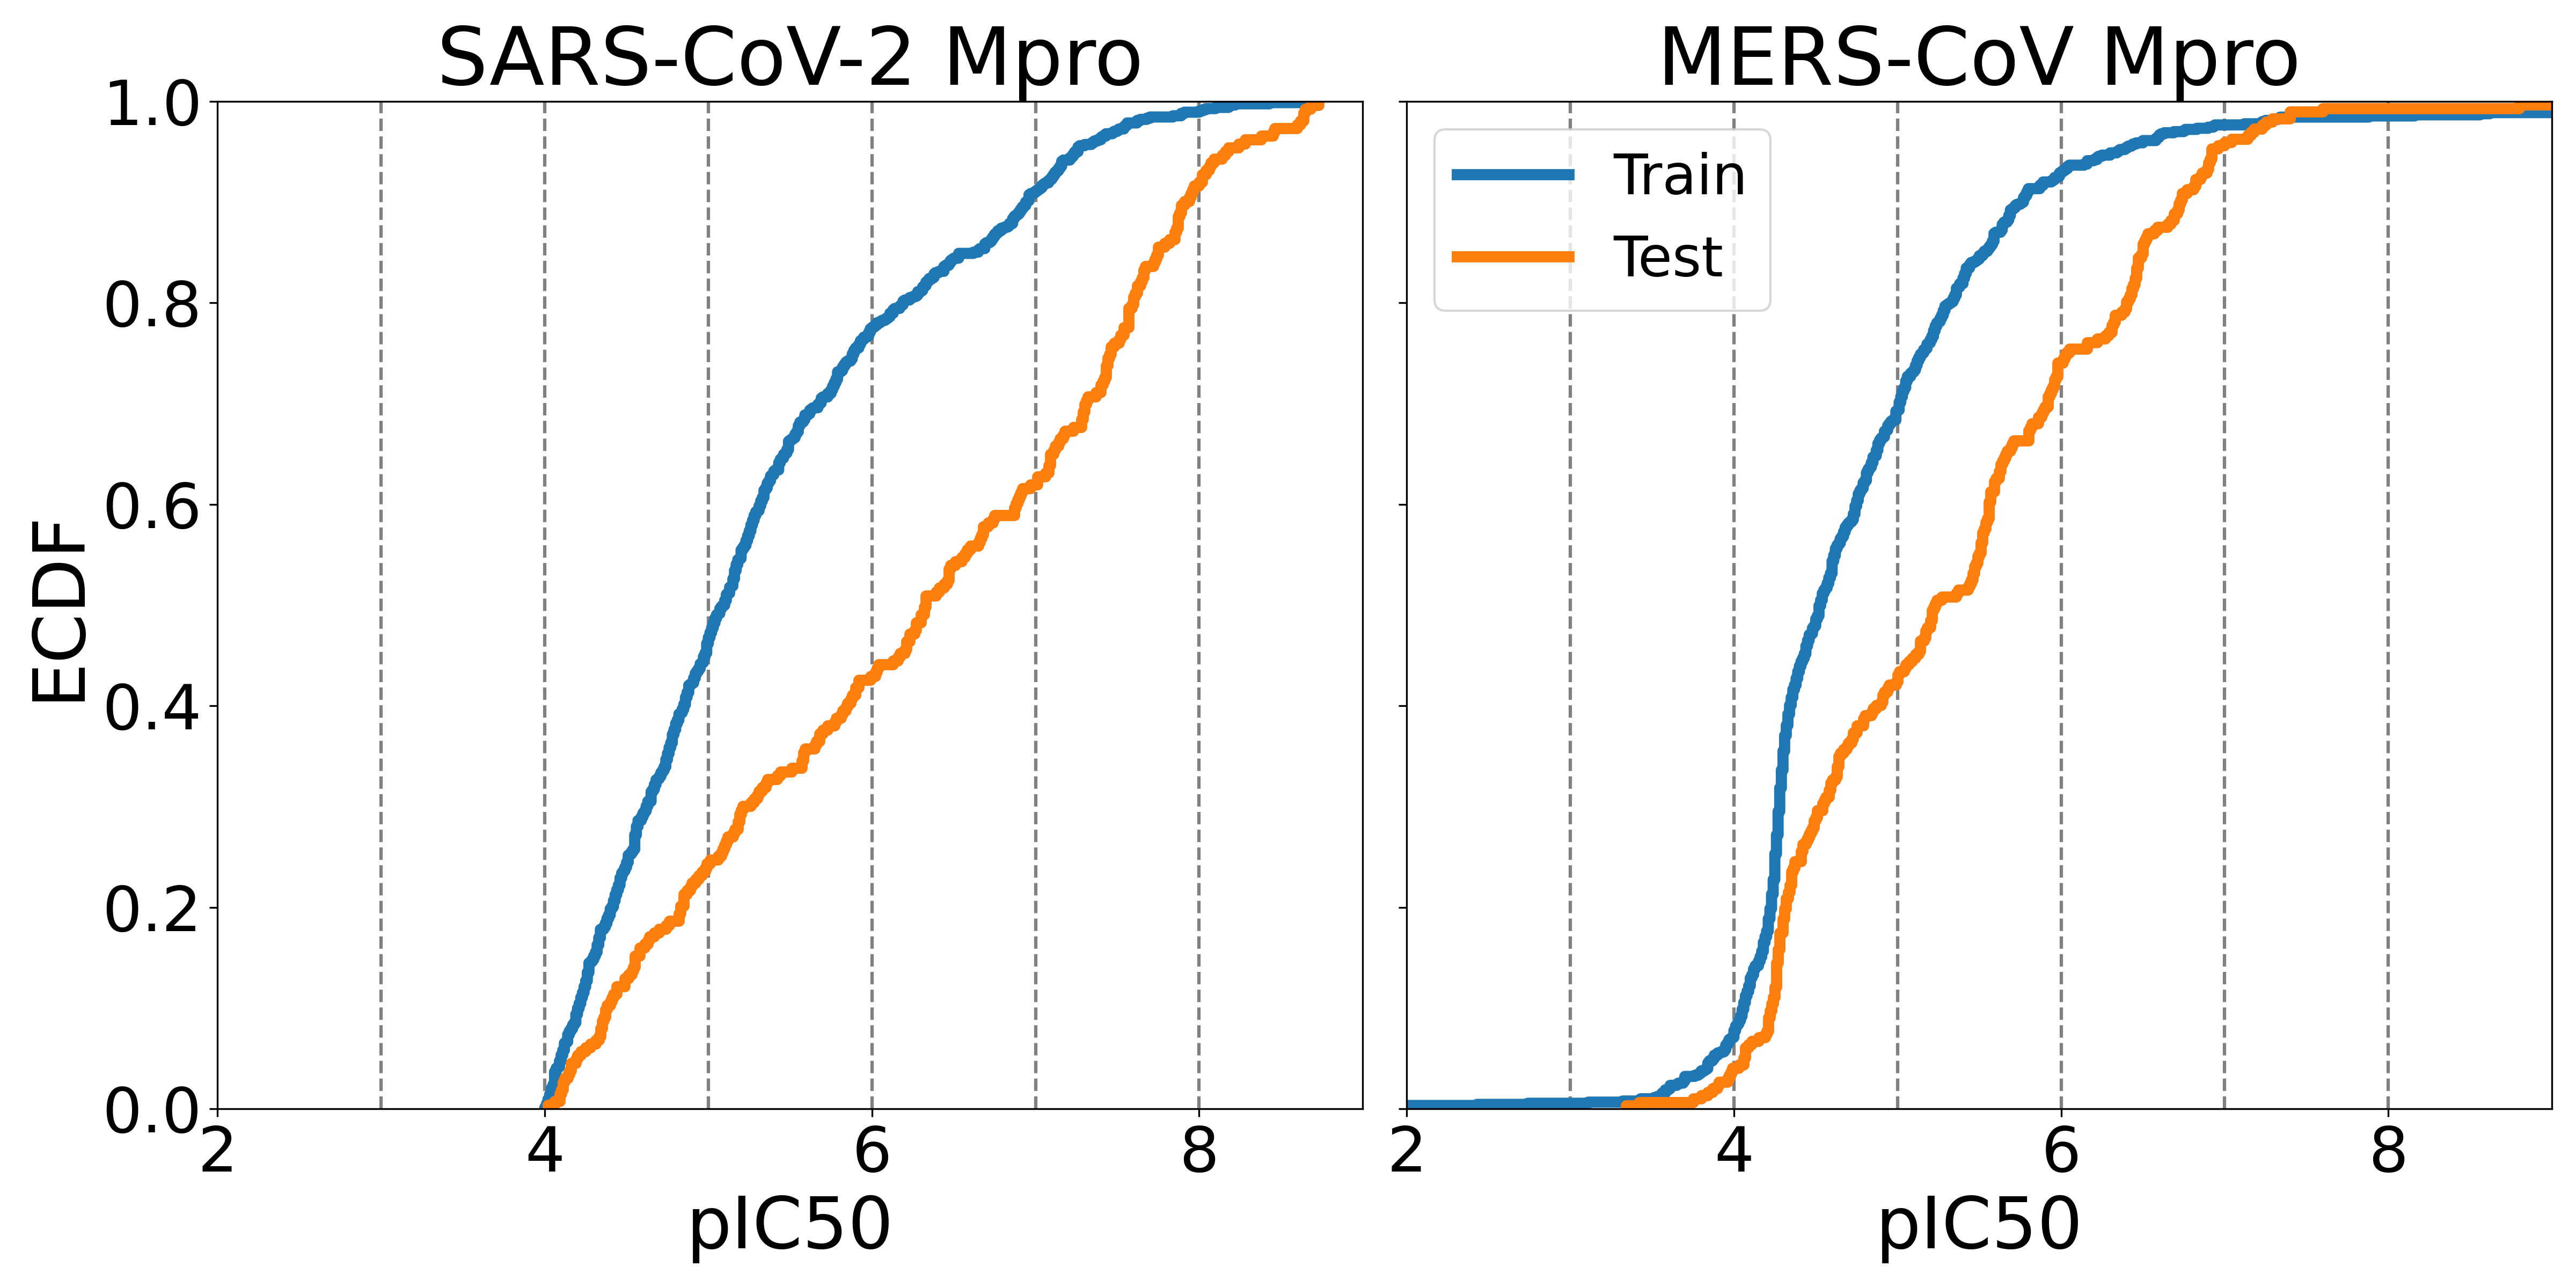
\includegraphics[scale=0.3]{SI/fig_S3_potency_dynamic_ranges/potency_dynamic_range.png}
  \caption{Distributions of dynamic ranges of biochemical potencies shown as Empirical Cumulative Distribution Functions (ECDFs). pIC50 values were fit from dose-response measurements as obtained by a Fluorescence Resonance Energy Transfer assay split between train set (blue) and test set (orange) and targets SARS-CoV-2 Mpro (left) and MERS-CoV Mpro (right). }
  \label{fgr:admet_endpoints}
\end{figure}



\begin{figure}
    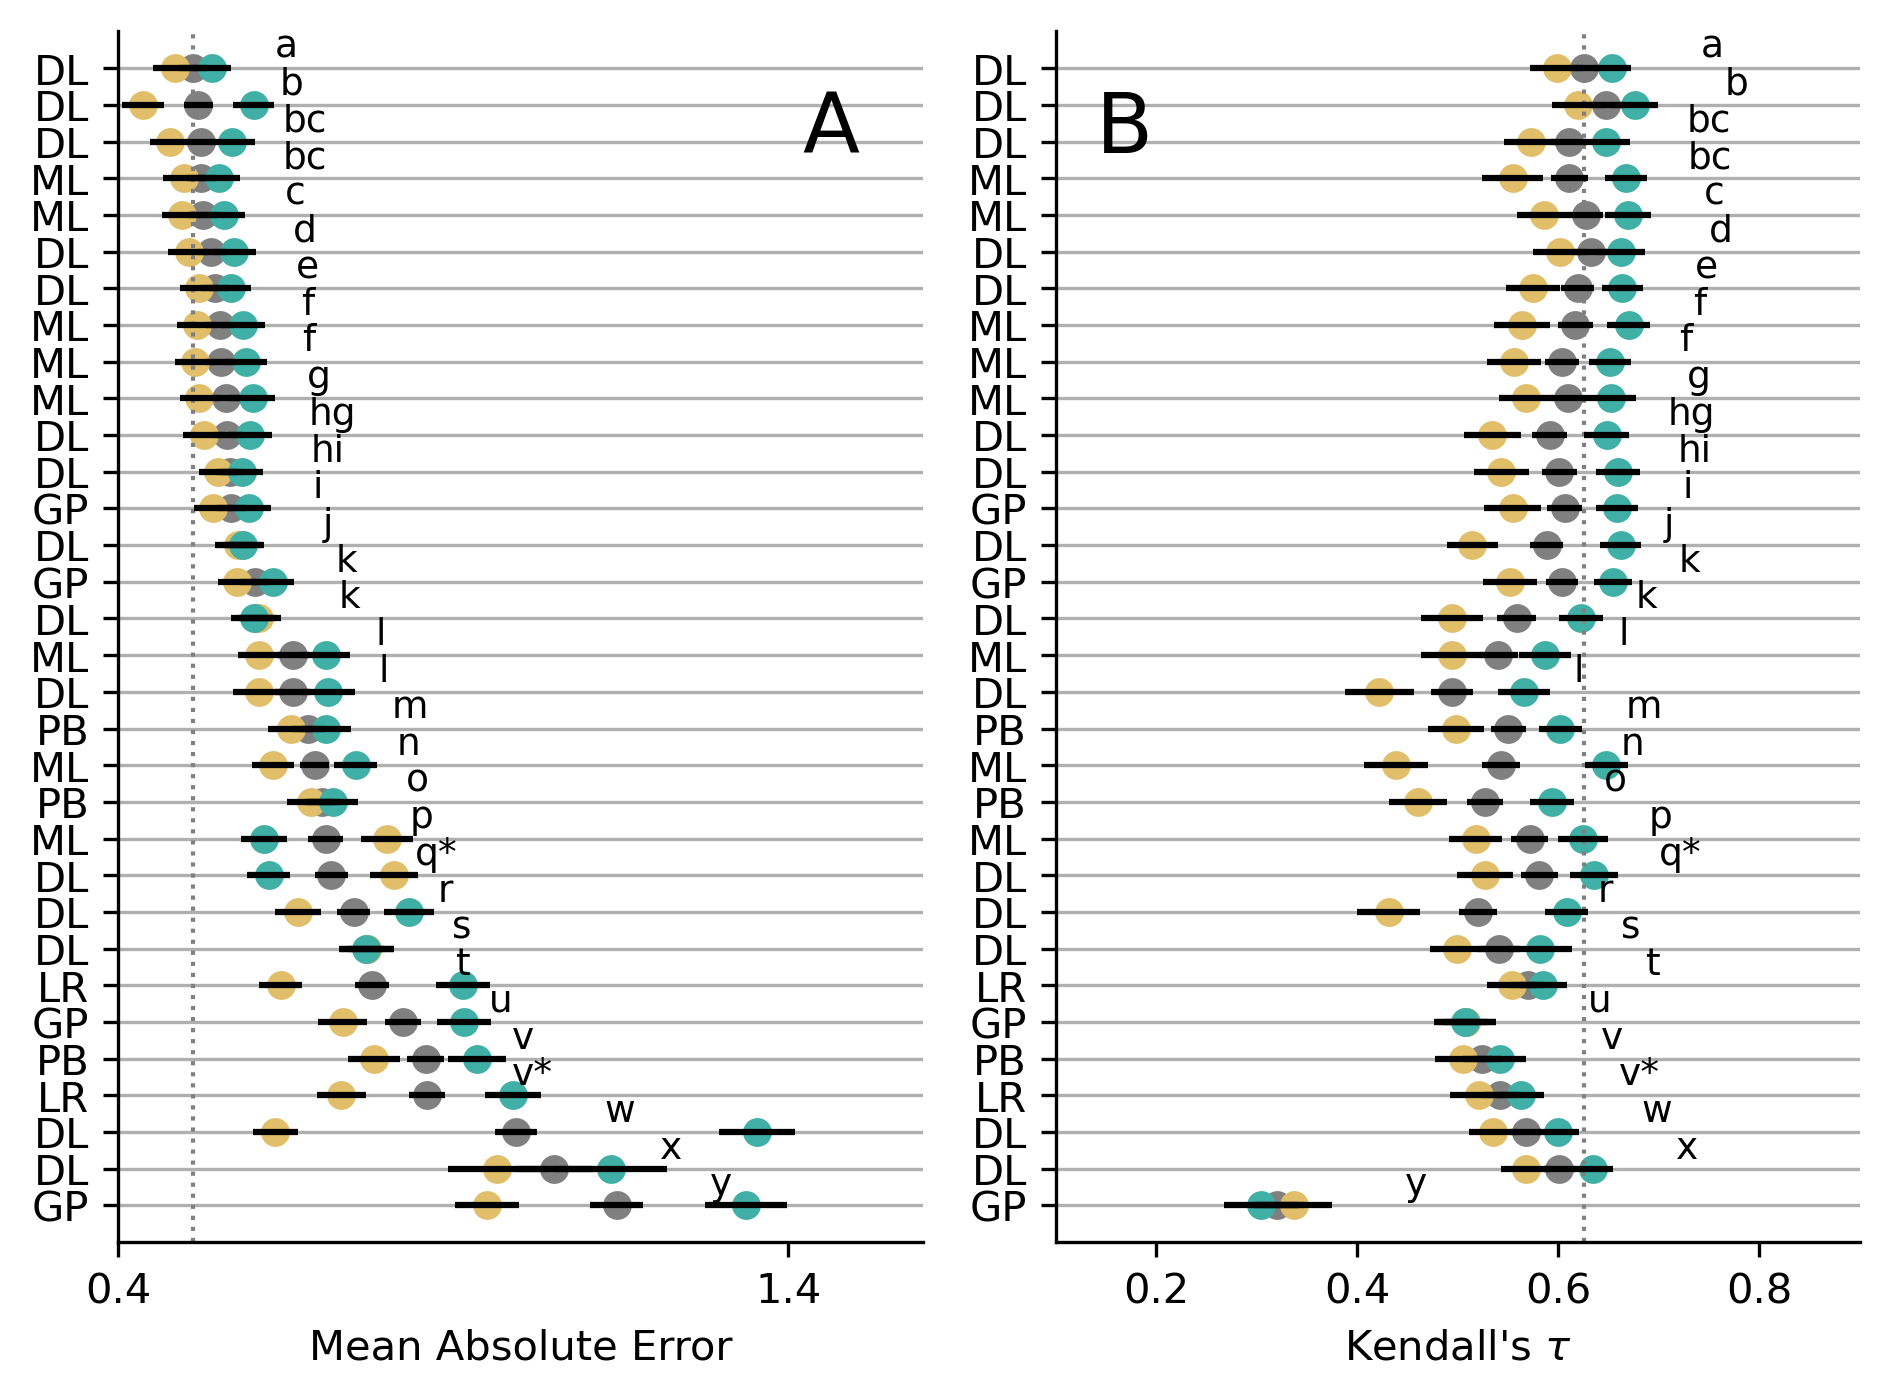
\includegraphics[scale=0.75]{SI/fig_S4_ktau_potency_leaderboard/SI_potency_leaderboards.png}
  \caption{Participants performed diversely on potency predictions. A) leaderboard of the potency subchallenge as each entry's category (DL=Deep Learning, ML=Machine Learning, PB=Physics-Based, GP=Gaussian Process, LR=Linear Regression) and split by target; MERS-CoV Mpro in yellow, SARS-CoV-2 Mpro in green). B) replication of panel A but using the ranking metric \textit{kendall's $\tau$ }. Baseline models as deployed by the organizers are marked with asterisks. Each entry is annotated with its statistical ranking by the Compact Letter Display (CLD) system.}
  \label{fgr:ktau_supp_potency}
\end{figure}



\begin{figure}
    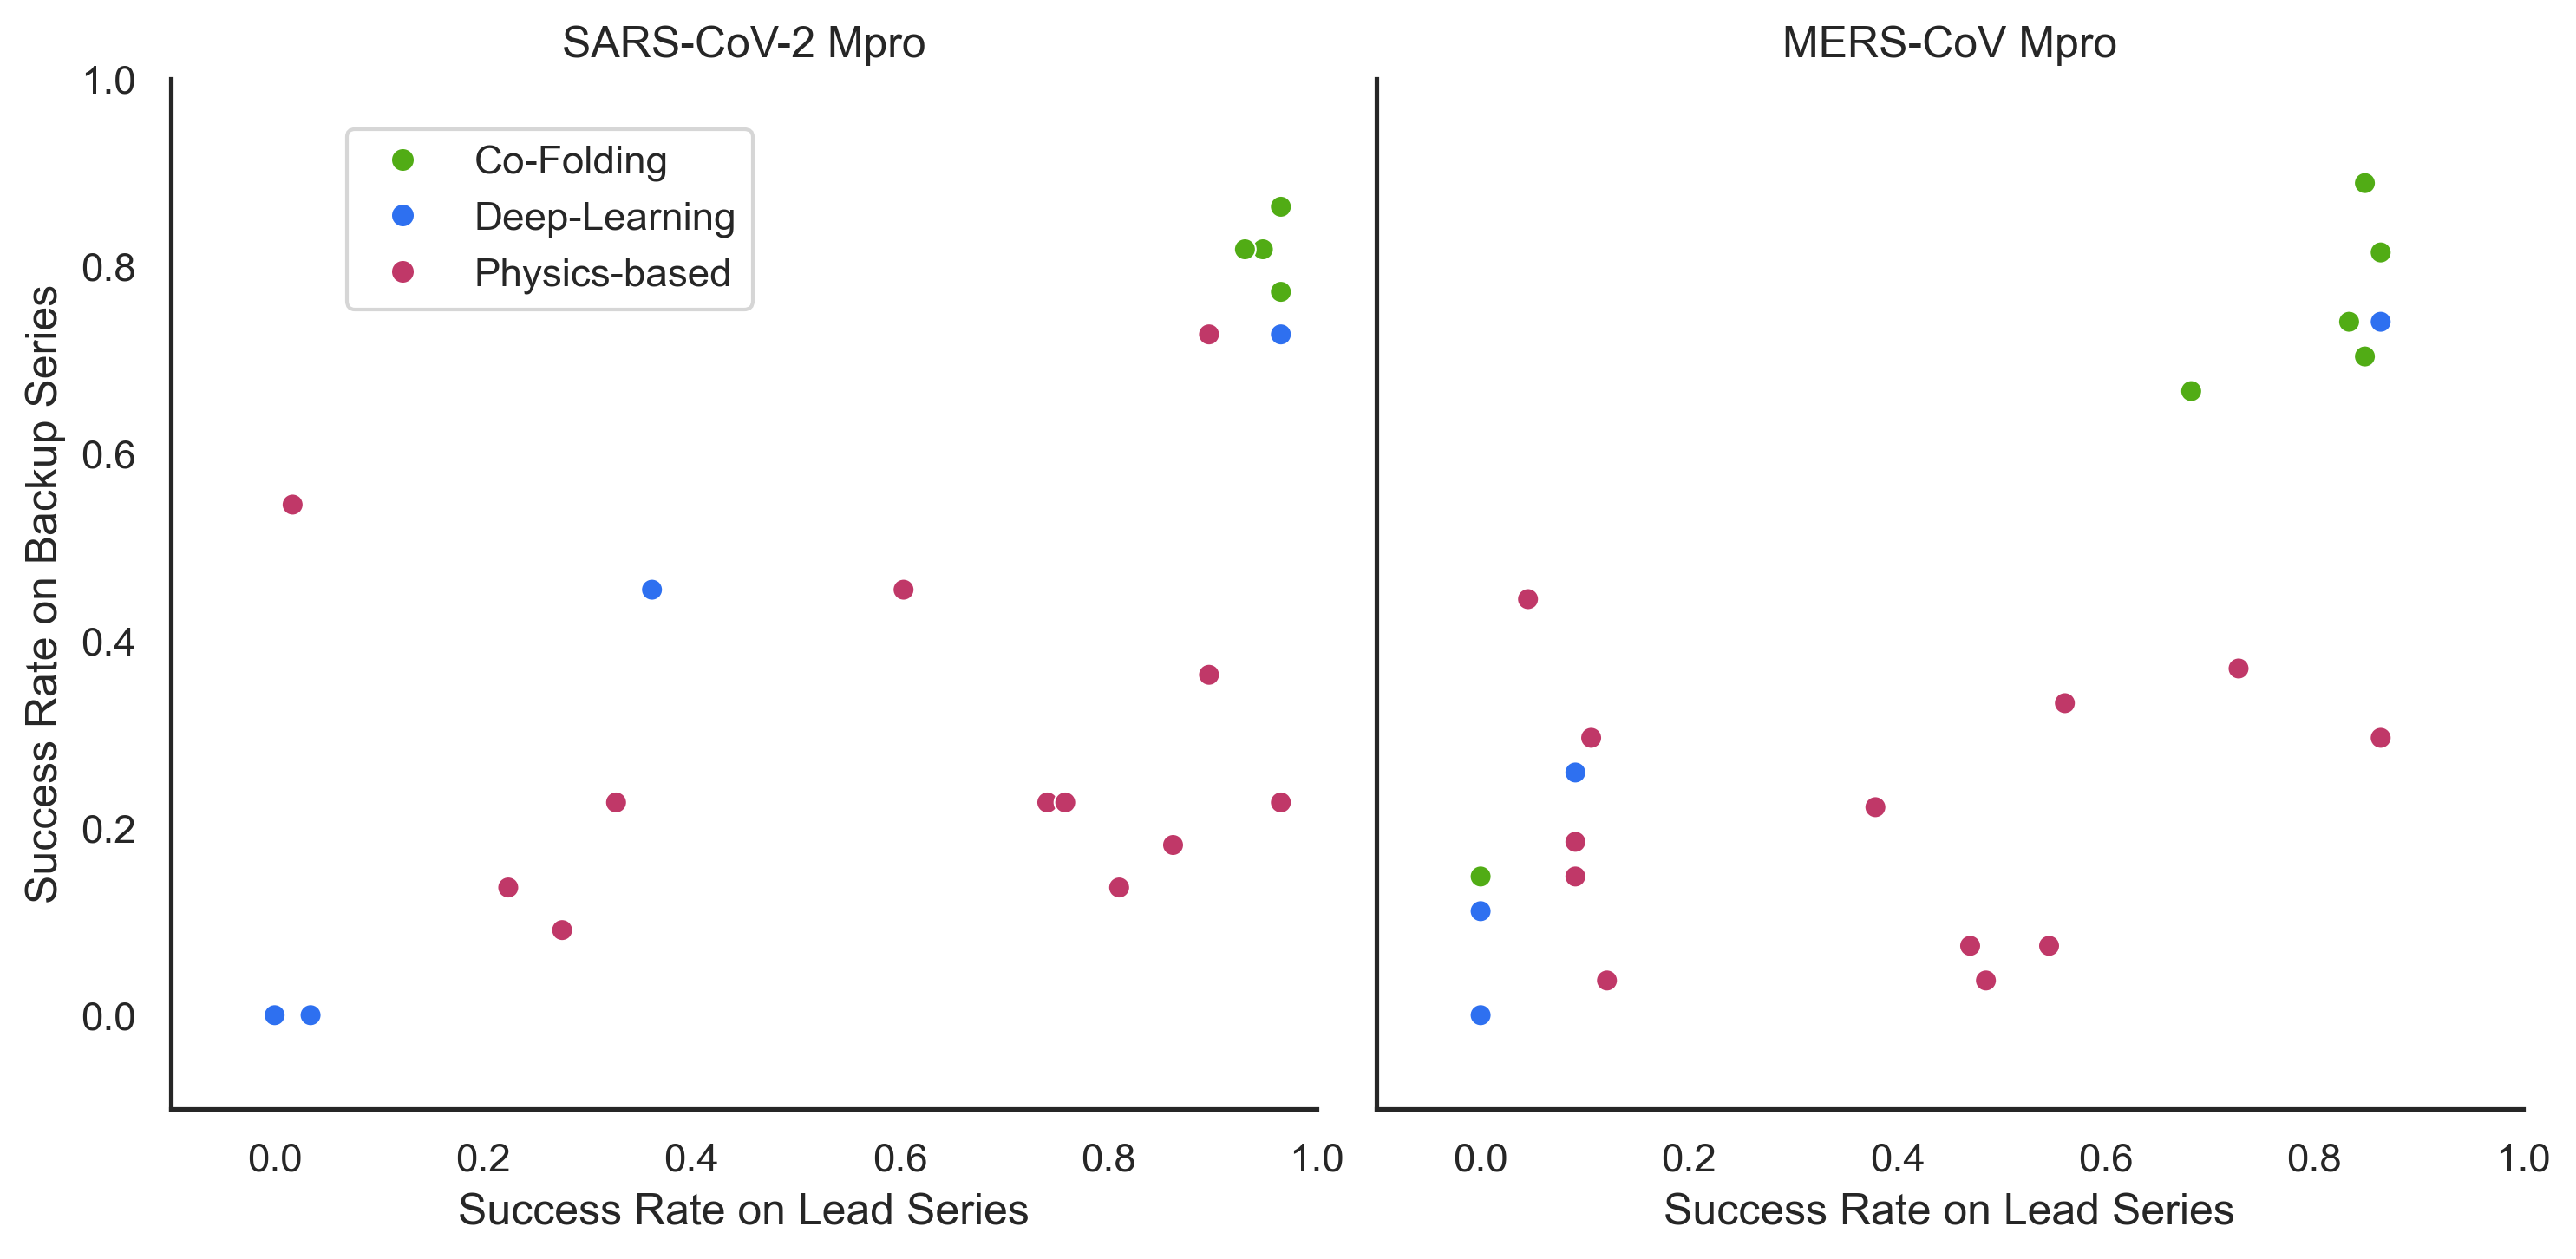
\includegraphics[scale=0.75]{SI/fig_S5_poses_by_series/success_rate_lead_vs_backup_comparison.png}
  \caption{Success rates of each type of model on the lead series vs backup series. This shows that the worse performance on the backup series comes mainly from the physics-based models, with the co-folding models doing well on both and the deep-learning doing poorly on both.}
  \label{fgr:success_rate_lead_vs_backup}
\end{figure}



% Please add the following required packages to your document preamble:
% \usepackage{multirow}
\newpage
\begin{table}[]
\begin{tabular}{lllll}
 &  &  & \multicolumn{2}{c}{Biochemical pIC50} \\ \cline{4-5} 
 & Isomer & Compound & SARS-CoV-2 Mpro & MERS-CoV Mpro \\
\multirow{2}{*}{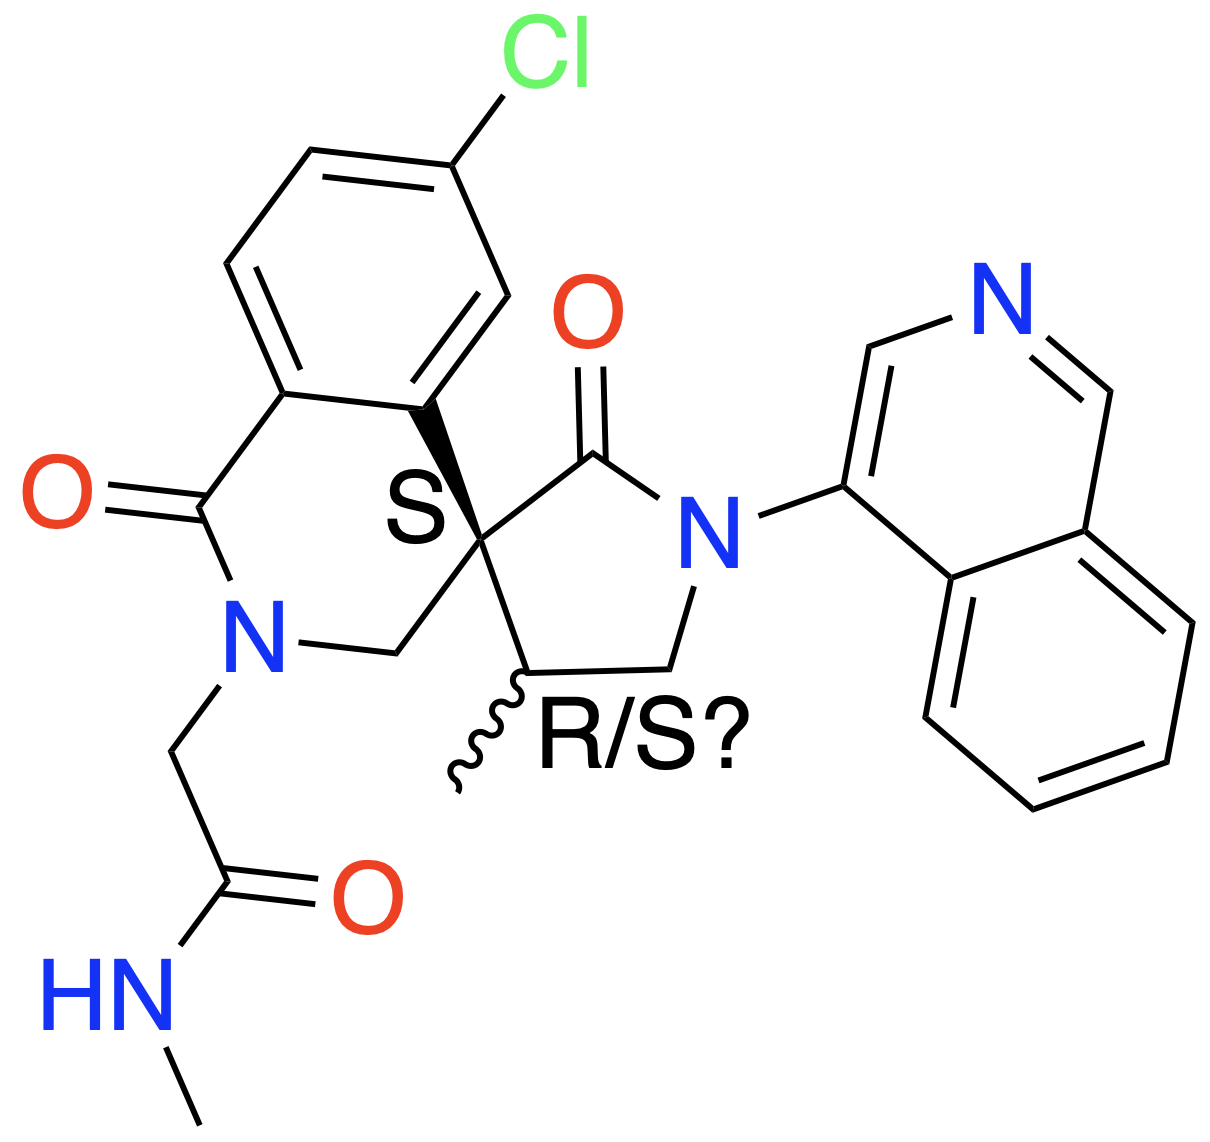
\includegraphics[scale=0.2]{SI/table_S1_stereoisomer_activity_cliffs/methyl.png}} & R & ASAP-0000733 & 7.87 & 5.97 \\
 & S & ASAP-0000240 & 5.62 & \textless 4.00 \\ \\ \\ \\ 
 \\ \\ \\ 
\multirow{2}{*}{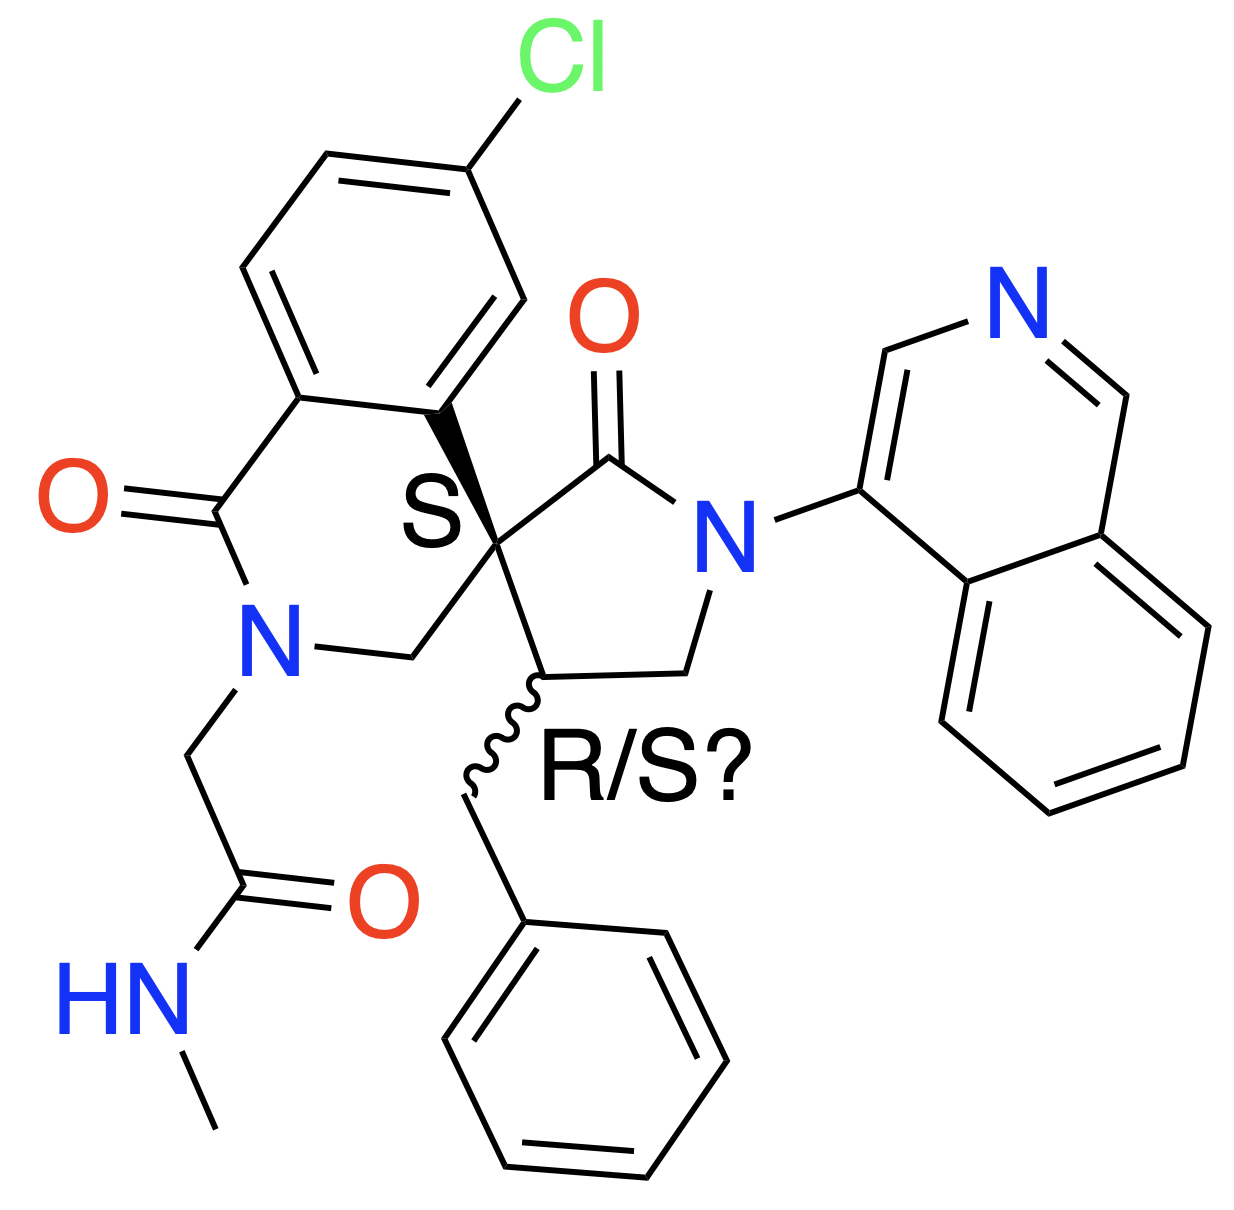
\includegraphics[scale=0.2]{SI/table_S1_stereoisomer_activity_cliffs/benzyl.png}} & R & ASAP-0000526 & 7.30 & 5.21 \\
 & S & ASAP-0000435 & 5.81 & \textless 4.00
\end{tabular}
\caption{Examples of large biochemical potency differences between chirally separated enantiomers of compounds involved in this blind challenge. Shown are the racemic structures with corresponding R/S enantiomers and their biochemical potencies in both SARS-CoV-2 Mpro and MERS-CoV Mpro. Values noted as \textless 4.0 are below the dynamic range of the assay.}
\end{table}


% \begin{sidewaystable}
% \tiny
%   \csvreader[tabular=|l|l|l|l|,
%   table head= \hline \textbf{Username} & \textbf{CLD} &  \textbf{MAE}  & \textbf{Report URL} \\ \hline,
%   respect underscore,
%   respect and,
%   head to column names,
%   late after line=\\\hline]{SI/potency_SI_table.csv}{}{\Username & \CLD & \MAE & \Report}%
% \caption{Performance of participants in the potency subchallenge with associated links to participant reports. Raw versions of this data is available at the paper GitHub repo: https://github.com/asapdiscovery/asap-blind-challenge-paper}
% \end{sidewaystable}


% \begin{sidewaystable}
% \tiny
%   \csvreader[tabular=|l|l|l|l|,
%   table head= \hline \textbf{Username} & \textbf{CLD} &  \textbf{MAE}  & \textbf{Report URL} \\ \hline,
%   respect underscore,
%   respect and,
%   head to column names,
%   late after line=\\\hline]{SI/admet_SI_table.csv}{}{\Username & \CLD & \MAE & \Report}%
% \caption{Performance of participants in the ADMET subchallenge with associated links to participant reports. Raw versions of this data is available at the paper GitHub repo: https://github.com/asapdiscovery/asap-blind-challenge-paper}
% \end{sidewaystable}


% \begin{sidewaystable}
% \tiny
%   \csvreader[tabular=|l|l|l|l|,
%   table head= \hline \textbf{Username} & \textbf{CLD} &  \textbf{MAE}  & \textbf{Report URL} \\ \hline,
%   respect underscore,
%   respect and,
%   head to column names,
%   late after line=\\\hline]{SI/ligand_pose_SI_table.csv}{}{\Username & \CLD & \MAE & \Report}%
% \caption{Performance of participants in the ligand pose subchallenge with associated links to participant reports. Raw versions of this data is available at the paper GitHub repo: https://github.com/asapdiscovery/asap-blind-challenge-paper}
% \end{sidewaystable}

\newpage

{\tiny

\begin{longtable}{|p{2cm}|c|c|c|p{4cm}|p{6cm}|}
\hline
\multicolumn{6}{|c|}{\small{\textbf{Potency}}} \\
\hline
\textbf{Username} & \textbf{CLD} & \textbf{Type} & \textbf{MAE} & \textbf{Github} & \textbf{Report} \\

\hline
\endfirsthead

\hline
\multicolumn{6}{|c|}{\small{\textbf{Potency}}} \\
\hline
\textbf{Username} & \textbf{CLD} & \textbf{Type} & \textbf{MAE} & \textbf{Github} & \textbf{Report} \\
\hline
\endhead

\endfoot

oscar-mendez-lucio & a & DL & 0.509 ± 0.022 & \url{https://github.com/recursionpharma/mole_public} & \url{https://www.nature.com/articles/s41467-024-53751-y} \\
\hline

ccorbi & b & DL & 0.516 ± 0.022 & \url{https://github.com/exscientia/molflux} & \url{https://gist.github.com/shug3502/f0fe74f443d1d82fa73bf869148c7cdc} \\
\hline

siat353 & b & ML & 0.517 ± 0.021 & & \url{https://drive.google.com/file/d/1axeFC3gxcVGKPDwVZO2Tyi7W9Mz2ztLN/view?usp=drive_link} \\
\hline

xubf & bc & DL & 0.518 ± 0.022 & & \url{https://docs.google.com/document/d/14NaFXBsCToKCyRTV2EiV7dTxBsBz_9R8ZWkTkLiovQk} \\
\hline

alx-dga & c & ML & 0.522 ± 0.022 & \url{https://github.com/alexisdougha/polaris-submission} & \url{https://drive.google.com/file/d/1jUPsolAyrgZ-mIxi5AAMYKBigjniNVCf/view?usp=sharing} \\
\hline

luispintoc & d & DL & 0.532 ± 0.022 & & \url{https://docs.google.com/document/d/124EmRMeXIZlXGmYmErVVvb5DLWnU_A_dXgwH43TAvvk/edit?usp=sharing} \\
\hline

ryan-deepmirror & e & DL & 0.539 ± 0.021 & \url{https://github.com/ryan-deepmirror} & \url{https://docs.google.com/document/d/1zFNA_CKfGRGbdzFXX8dOhkLIOFBybe6pn3H7X8qd6nY/edit?usp=sharing} \\
\hline

rced & f & ML & 0.544 ± 0.022 & \url{https://github.com/cedenoruel/sub_antiviral25} & \url{https://github.com/cedenoruel/sub_antiviral25} \\
\hline

dodo & f & ML & 0.548 ± 0.022 & \url{https://github.com/fulopjoz/polaris-antiviral-submission/blob/master/potency-submission/potency-prediction-pipeline.ipynb} & \url{https://tinyurl.com/dodo-potency} \\
\hline

sina & g & ML & 0.554 ± 0.021 & & \url{https://github.com/khosravisina/Polaris-potency-report/tree/main} \\
\hline

gufan1998 & g & DL & 0.555 ± 0.022 & \url{https://github.com/gu-yaowen/GGAP-CPI} & \url{https://docs.google.com/document/d/1B2I1pnHB32qy_CmbFXAWgNfNG-4qn_C2/edit?usp=sharing&ouid=108734974888240888578&rtpof=true&sd=true} \\
\hline

wim0 & h & DL & 0.561 ± 0.021 & \url{https://github.com/dehaenw/polaris-baseline} & \url{https://molecular.beauty/blog/2025/03/13/polaris.html} \\
\hline

austint & h & GP & 0.564 ± 0.021 & \url{https://github.com/AustinT/asap-2025-challenge-gp} & \url{https://github.com/AustinT/asap-2025-challenge-gp} \\
\hline

jacksonburns & i & DL & 0.575 ± 0.022 & \url{https://github.com/JacksonBurns/neural-pairwise-regression/blob/main/notebooks/polaris_asap.ipynb} & \url{https://github.com/JacksonBurns/neural-pairwise-regression/blob/main/meta} \\
\hline

caithmac & j & GP & 0.600 ± 0.021 & & \url{https://github.com/caithmac/polaris_potency_mpro} \\
\hline

talagayev & j & DL & 0.602 ± 0.024 & \url{https://github.com/talagayev/polaris_antiviral_challenge} & \url{https://github.com/talagayev/polaris_antiviral_challenge/blob/main/ADMET_MPNN/report.md} \\
\hline

steffen-wedig & k & DL & 0.656 ± 0.028 & & \url{https://drive.google.com/file/d/1ZkPnvkzNaEYe45fLpGZyNUvU9rnM_oDq/view?usp=sharing} \\
\hline

wolberlab & k & ML & 0.660 ± 0.024 & \url{https://github.com/talagayev/polaris_antiviral_challenge} & \url{https://github.com/talagayev/polaris_antiviral_challenge/blob/main/Preliminary_prediction_protocol_2nd_submission.md} \\
\hline

nnnty & l & PB & 0.676 ± 0.025 & & \url{https://github.com/yul533/polaris-antiviral-challenge/blob/main/potency%20prediction%202} \\
\hline

azminewasi & m & ML & 0.687 ± 0.022 & \url{https://github.com/azminewasi/polaris-antiviral-competition} & \url{https://github.com/azminewasi/polaris-antiviral-competition/blob/main/antiviral-potency-2025/report/report.pdf} \\
\hline

yul533 & n & PB & 0.697 ± 0.025 & & \url{https://github.com/yul533/polaris-antiviral-challenge/blob/main/potency%20prediction} \\
\hline

wtrd & o & ML & 0.702 ± 0.026 & \url{https://github.com/duartegroup/asap-polaris-challenge} & \url{https://docs.google.com/document/d/1464wiMCWdncfWoMIpL4WHI31qOECqeBq0CEhwiAAfW4/edit?usp=sharing} \\
\hline

bkaminow & p* & DL & 0.712 ± 0.024 & \url{https://github.com/kaminow/asap-polaris-challenge-potency-2025} & \url{https://github.com/kaminow/asap-polaris-challenge-potency-2025/blob/main/report.md} \\
\hline

kysun & q & DL & 0.748 ± 0.026 & \url{https://github.com/KSUN63/Polaris-Submission} & \url{https://docs.google.com/document/d/1YVxVi-zMc7rX0TrvO7SIZfkQ-uUx3ChdtV4oovq80ts/edit?usp=sharing} \\
\hline

longhung25 & r & DL & 0.764 ± 0.029 & & \url{https://docs.google.com/document/d/140sY_Rx_YPEnaw4TbuvuuaO4rq1F29TvNHh779Me5Jc/edit?usp=sharing} \\
\hline

danialshah353 & s & LR & 0.772 ± 0.026 & & \url{https://drive.google.com/file/d/1xrmgHAFcyRDAGTQTEeHn83GxuQBfm4cr/view?usp=sharing} \\
\hline

hbaumann & t & GP & 0.822 ± 0.027 & & \url{https://github.com/meyresearch/polaris_challenge/tree/main} \\
\hline

kbishop & u & PB & 0.853 ± 0.030 & & \url{https://docs.google.com/document/d/1exokoYptuwRllvnQp_S42ZW3ecDc6zdk/edit?usp=sharing&ouid=111958341380201258210&rtpof=true&sd=true} \\
\hline

hmacdope & u* & LR & 0.857 ± 0.027 & & \url{https://github.com/asapdiscovery/asap-polaris-challenge-baselines} \\
\hline

kriegegroup & v & DL & 0.990 ± 0.032 & \url{https://github.com/aehrlich1/polaris-challenge-2025} & \url{https://docs.google.com/document/d/1mth0dsjh6ir_qEQt-3CW7YsZHR1LK2jF6rsguKbd89M/edit?usp=sharing} \\
\hline

geosmina & w & DL & 1.053 ± 0.056 & & \url{https://github.com/jaaisu/polaris_challenge/blob/main/README.md} \\
\hline

ialibay & x & GP & 1.146 ± 0.039 & \url{https://github.com/meyresearch/polaris_challenge/tree/potency} & \url{https://github.com/meyresearch/polaris_challenge/tree/main} \\
\hline


\caption{Performance of participants in the potency subchallenge with associated links to participant reports. Raw versions of this data is available at the paper GitHub repo: \url{https://github.com/asapdiscovery/asap-blind-challenge-paper}}
\label{tab:admet_results}
\end{longtable}
}


\newpage




\newpage
{\tiny

\begin{longtable}{|p{2cm}|c|c|c|p{4cm}|p{6cm}|}
\hline
\multicolumn{6}{|c|}{\small{\textbf{ADMET}}} \\
\hline
\textbf{Username} & \textbf{CLD} & \textbf{Type} & \textbf{MAE} & \textbf{Github} & \textbf{Report} \\
\hline
\endfirsthead

\hline
\multicolumn{6}{|c|}{\small{\textbf{ADMET}}} \\
\hline
\textbf{Username} & \textbf{CLD} & \textbf{Type} & \textbf{MAE} & \textbf{Github} & \textbf{Report} \\
\hline
\endhead

\endfoot


prairiewarbler10 & a & DL & 0.224 ± 0.009 & & \url{https://docs.google.com/document/d/1pof60W0rzZzhGYBxdtclGiq3TdZwtPVqB7Os2xTD8Us/edit?tab=t.0} \\
\hline


ebl88 & b & DL & 0.243 ± 0.009 & & \url{https://docs.google.com/document/d/1A6sRjezd7GSeLatF7VTE9NeFhmA4rSzmgTvZTL1_Nh4/edit?usp=sharing} \\
\hline


vchupakhin & c & ML & 0.269 ± 0.010 & & \url{https://gist.github.com/vchupakhinspl/9a5583d6acb9c1d1613a38710fefbbf6} \\
\hline


longhung25 & d & DL & 0.276 ± 0.010 & & \url{https://docs.google.com/document/d/1WBi1vd4_w09FliNxQ01vYq9j8mbzwHYqLtW0k_fUWlU/edit?usp=sharing} \\
\hline


xiaolinpan & de & DL & 0.277 ± 0.010 & & \url{https://docs.google.com/document/d/1BzIMfdOfXJMHmuIfnlQUZRCnVfqNQKzgXZbnpJZBFwI/edit?usp=sharing} \\
\hline


weijunzhou & e & DL & 0.279 ± 0.010 & \url{https://github.com/WeiJunZhou23/MolMCL.git} & \url{https://docs.google.com/document/d/1TPsdWO654-tL_Lz4_b_66xdGPeGNglil/edit?usp=drive_link&ouid=104987191201424644843&rtpof=true&sd=true} \\
\hline


ryan-deepmirror & f & DL & 0.291 ± 0.010 & \url{https://github.com/ryan-deepmirror} & \url{https://docs.google.com/document/d/1zFNA_CKfGRGbdzFXX8dOhkLIOFBybe6pn3H7X8qd6nY/edit?usp=sharing} \\
\hline


rced & f & ML & 0.292 ± 0.010 & \url{https://github.com/cedenoruel/sub_antiviral25} & \url{https://github.com/cedenoruel/sub_antiviral25} \\
\hline


luispintoc & g & DL & 0.301 ± 0.010 & & \url{https://docs.google.com/document/d/124EmRMeXIZlXGmYmErVVvb5DLWnU_A_dXgwH43TAvvk/edit?usp=sharing} \\
\hline


oscar-mendez-lucio & h & DL & 0.307 ± 0.010 & \url{https://github.com/recursionpharma/mole_public} & \url{https://www.nature.com/articles/s41467-024-53751-y} \\
\hline


vladvin & i & DL & 0.315 ± 0.013 & \url{https://github.com/Alicegaz/AgenticADMET} & \url{https://docs.google.com/document/d/16y9EtElTmJ-p0bAYjJaNgkU8WP-CYz77lhHB2oxkTc4/edit?usp=sharing} \\
\hline


qb2025 & i & ML & 0.316 ± 0.010 & & \url{https://docs.google.com/document/d/118YhHzl7rEyoAwYSdiRxWzS_7RmweZbDyDFNHzlSTzo/edit?usp=drive_link} \\
\hline


xubf & i & DL & 0.317 ± 0.012 & & \url{https://docs.google.com/document/d/14NaFXBsCToKCyRTV2EiV7dTxBsBz_9R8ZWkTkLiovQk} \\
\hline


dzqh & j & ML & 0.320 ± 0.011 & & \url{https://drive.google.com/file/d/11JPTjWpcehLFpgmo9jpcJXyurLSvpTqm/view?usp=sharing} \\
\hline


jharrison & k & DL & 0.323 ± 0.011 & \url{https://github.com/exscientia/molflux} & \url{https://gist.github.com/shug3502/f0fe74f443d1d82fa73bf869148c7cdc} \\
\hline


haleemiliyash & l & ML & 0.329 ± 0.011 & \url{https://github.com/haleemiliyash/ASAP-polaris-blind-challenge-Ligand-ADMET-property-prediction-.git} & \url{https://docs.google.com/document/d/1fAZjJBSr3RDBXpZQNv_tcGKWohCIrPdUZYNf1ku1bYo/edit?usp=sharing} \\
\hline


alx-dga & l & ML & 0.329 ± 0.011 & \url{https://github.com/alexisdougha/polaris-submission} & \url{https://drive.google.com/file/d/1jUPsolAyrgZ-mIxi5AAMYKBigjniNVCf/view?usp=sharing} \\
\hline


austint & m & GP & 0.334 ± 0.012 & \url{https://github.com/AustinT/asap-2025-challenge-gp} & \url{https://github.com/AustinT/asap-2025-challenge-gp} \\
\hline


adavi & m & DL & 0.335 ± 0.012 & & \url{https://storage.polarishub.io/2025-01-asap-discovery/reports/adavi.pdf} \\
\hline


steffen-wedig & n & DL & 0.347 ± 0.013 & & \url{https://drive.google.com/file/d/1ZkPnvkzNaEYe45fLpGZyNUvU9rnM_oDq/view?usp=sharing} \\
\hline


jacksonburns & o & DL & 0.350 ± 0.014 & \url{https://github.com/JacksonBurns/neural-pairwise-regression/blob/main/notebooks/polaris_asap.ipynb} & \url{https://github.com/JacksonBurns/neural-pairwise-regression/blob/main/meta} \\
\hline


dodo & o & ML & 0.352 ± 0.012 & \url{https://github.com/fulopjoz/polaris-antiviral-submission/blob/master/admet-submission/admet_pipeline_b.ipynb} & \url{https://tinyurl.com/dodo-admet} \\
\hline


balamuruganthirukonda & p & ML & 0.359 ± 0.013 & \url{https://github.com/BalamuruganThirukonda/Polaris_competition.git} & \url{https://docs.google.com/document/d/1lfroAm0TW4mxhHkZjAngHVioe5vrmQMp2C6TzWinu_g/edit?usp=sharing} \\
\hline


wvirany & q & GP & 0.369 ± 0.013 & \url{https://github.com/wvirany} & \url{https://github.com/wvirany/BayesOpt} \\
\hline


azminewasi & r & DL & 0.396 ± 0.013 & \url{https://github.com/azminewasi/polaris-antiviral-competition} & \url{https://github.com/azminewasi/polaris-antiviral-competition/blob/main/antiviral-admet-2025/report/report.pdf} \\
\hline


wolberlab & s & DL & 0.416 ± 0.013 & \url{https://github.com/talagayev/polaris_antiviral_challenge} & \url{https://github.com/talagayev/polaris_antiviral_challenge/blob/main/ADMET_MPNN/report.md} \\
\hline


agitter & t & DL & 0.418 ± 0.016 & \url{https://github.com/agitter/asap-polaris-admet-challenge} & \url{https://doi.org/10.5281/zenodo.14993394} \\
\hline


hmacdope & u* & LR & 0.430 ± 0.011 & & \url{https://github.com/asapdiscovery/asap-polaris-challenge-baselines} \\
\hline


wtrd & u & ML & 0.430 ± 0.014 & \url{https://github.com/duartegroup/asap-polaris-challenge} & \url{https://docs.google.com/document/d/1464wiMCWdncfWoMIpL4WHI31qOECqeBq0CEhwiAAfW4/edit?usp=sharing} \\
\hline


ashmita-bose & v & ML & 0.444 ± 0.016 & & \url{https://github.com/AshmitaBose/Polaris-ADMET-ASHMITA-BOSE.git} \\
\hline


wim0 & v & DL & 0.444 ± 0.014 & \url{https://github.com/dehaenw/polaris-baseline} & \url{https://molecular.beauty/blog/2025/03/13/polaris.html} \\
\hline


ppxasjsm & w & DL & 0.504 ± 0.014 & \url{https://github.com/meyresearch/polaris_challenge/} & \url{https://github.com/meyresearch/polaris_challenge/blob/main/admet/report.md} \\
\hline


yul533 & x & DL & 0.513 ± 0.016 & & \url{https://github.com/yul533/polaris-antiviral-challenge/blob/main/admet%20prediction} \\
\hline


apalania & y & DL & 0.548 ± 0.019 & & \url{https://github.com/apalania/Polaris_ASAP-Challenge-2025/blob/main/Report.pdf} \\
\hline


hugo-oicr-quaccel & z & DL & 0.615 ± 0.015 & & \url{https://docs.google.com/document/d/1NzwitQ-LugGcRjqfumZrAQQi-Wy1kEVC4U1-Rmfty9k/edit?usp=sharing} \\
\hline


talagayev & A & DL & 0.663 ± 0.014 & \url{https://github.com/talagayev/polaris_antiviral_challenge} & \url{https://github.com/talagayev/polaris_antiviral_challenge/blob/main/ADMET_MPNN/report.md} \\
\hline


kushal & B & ML & 1.106 ± 0.020 & & \url{http://storage.polarishub.io/2025-01-asap-discovery/reports/kushal.docx} \\
\hline


cc25 & C & DL & 1.277 ± 0.018 & & \url{https://docs.google.com/document/d/1wwmnhGN82uaxNyC3Mr5kj5fCGb_bQ7wT/edit?usp=sharing&ouid=112042337312439931657&rtpof=true&sd=true} \\
\hline


kriegegroup & D & DL & 1.338 ± 0.020 & \url{https://github.com/aehrlich1/polaris-challenge-2025} & \url{https://docs.google.com/document/d/1mth0dsjh6ir_qEQt-3CW7YsZHR1LK2jF6rsguKbd89M/edit?usp=sharing} \\
\hline


\caption{Performance of participants in the ADMET subchallenge with associated links to participant reports. Raw versions of this data is available at the paper GitHub repo: \url{https://github.com/asapdiscovery/asap-blind-challenge-paper}}
\label{tab:admet_results}
\end{longtable}
}


\newpage



%% POSES

{\tiny

\begin{longtable}{|p{2cm}|c|c|c|p{4cm}|p{6cm}|}
\hline
\multicolumn{6}{|c|}{\small{\textbf{Ligand Poses}}} \\
\hline
\textbf{Username} & \textbf{CLD} & \textbf{Type} & \textbf{MAE} & \textbf{Github} & \textbf{Report} \\
\hline
\endfirsthead

\hline
\multicolumn{6}{|c|}{\small{\textbf{ADMET}}} \\
\hline
\textbf{Username} & \textbf{CLD} & \textbf{Type} & \textbf{Sucess Rate} & \textbf{Github} & \textbf{Report} \\
\hline
\endhead

\endfoot

averkova-nika98 & a+ & CF & 86.378 ± 2.466 &   & \url{https://docs.google.com/document/d/1SGw3gklEnCv-n_zV3mRvpl4sok304032/edit} \\
\hline
ernestglukhov & b+ & CF & 85.363 ± 2.603 &   & \url{https://docs.google.com/document/d/1ZscH4iBQFIDemyQVkfVfAevUrpPBmJ-vUiBYwwhMAK0/edit} \\
\hline
vemikainen & b+ & CF & 85.213 ± 2.601 &   & \url{https://docs.google.com/document/d/1e4ot7699vR7WfHQoaUXe7tRv7gN127Eu/edit} \\
\hline
vemikainenalt & c+ & DL & 84.673 ± 2.670 &   & \url{https://docs.google.com/document/d/1QujhEKtMpdUwFxE_AVq6RBzsHEh4gjkd/edit} \\
\hline
wiwnopgm & d & CF & 83.657 ± 2.769 &   & \url{https://apricot-zorah-51.tiiny.site} \\
\hline
auro & e & CF & 73.283 ± 3.368 & \url{https://github.com/meyresearch/polaris_challenge} & \url{https://github.com/meyresearch/BoltzForPolaris/blob/...} \\
\hline
hmacdope & f* & PB & 67.277 ± 3.453 &   & \url{https://github.com/asapdiscovery/asap-polaris-challenge-baselines} \\
\hline
rced & g & PB & 62.475 ± 3.583 & \url{https://github.com/cedenoruel/sub_antiviral25} & \url{https://github.com/cedenoruel/sub_antiviral25} \\
\hline
kysun & h & PB & 53.138 ± 3.686 & \url{https://github.com/KSUN63/Polaris-Submission} & \url{https://docs.google.com/document/d/1YVxVi-zMc7rX0TrvO7SIZfkQ-uUx3ChdtV4oovq80ts/edit} \\
\hline

jthorton & i & PB & 48.136 ± 3.703 & \url{https://github.com/jthorton/polaris_fegrow_mcs} & \url{https://github.com/jthorton/polaris_fegrow_mcs} \\
\hline

djc56 & j & PB & 47.176 ± 3.767 & \url{https://github.com/cole-group/FEgrow} & \url{https://github.com/cole-group/polaris-fegrow} \\
\hline

kbishop & k & PB & 40.984 ± 3.657 &   & \url{https://docs.google.com/document/d/1exokoYptuwRllvnQp_S42ZW3ecDc6zdk/edit} \\
\hline

ryusei-ogino & l & PB & 40.028 ± 3.720 &   & \url{https://github.com/ryusei-ogino/antiviral-challenge} \\
\hline

wim0 & m & PB & 34.553 ± 3.600 & \url{https://github.com/dehaenw/polaris-baseline} & \url{https://molecular.beauty/blog/2025/03/13/polaris.html} \\
\hline

xuhangdai & n & DL & 29.415 ± 3.204 & \url{https://github.com/XDaiNYU/} & \url{https://docs.google.com/document/d/e/2PACX-1vQueWu4Myu0YAguHKRHMX88y7vl4_8z-6_2Y0UX...} \\
\hline

yul533 & o & PB & 25.785 ± 3.171 &   & \url{https://github.com/yul533/polaris-antiviral-challenge/blob/main/pose prediction} \\
\hline

dodo & p & PB & 22.442 ± 2.990 & \url{https://github.com/fulopjoz/polaris-antiviral-submission} & \url{https://tinyurl.com/dodo-poses} \\
\hline

fjclark & q & PB & 18.548 ± 2.915 & \url{https://github.com/michellab/polaris-poses-challenge-fegrow-a3fe} & \url{https://github.com/michellab/polaris-poses-challenge-fegrow-a3fe} \\
\hline

myzzzz & r & PB & 17.391 ± 2.778 & \url{https://github.com/myzzzz6} & \url{https://www.quantabricks.xyz} \\
\hline

nnnty & s & PB & 16.349 ± 2.668 &   & \url{https://github.com/yul533/polaris-antiviral-challenge/blob/main/pose prediction 2} \\
\hline

jscheen & t* & CF & 2.681 ± 1.161 &   & \url{https://github.com/asapdiscovery/asap-polaris-challenge-baselines} \\
\hline

vanguard737 & u & DL & 2.174 ± 1.089 & \url{https://github.com/alpha29/polaris-asap-poses} & \url{https://github.com/alpha29/polaris-asap-poses/blob/master/doc/report.md} \\
\hline

kriegegroup & v & DL & 1.110 ± 0.765 & \url{https://github.com/ellenaj0/polaris-challenge-ligand-poses-2025} & \url{https://drive.google.com/file/d/1leKiDHVeGDe5GL0_ll8fxZrDh05d4X7g/view} \\
\hline

sekuen & w & DL & 0.000 ± 0.000 &   & \url{https://colab.research.google.com/drive/1lne8e6-4gkNb3HwocvWBOH6NUBX0svc4} \\
\hline

\caption{Performance of participants in the Ligand Pose subchallenge with associated links to participant reports. Raw versions of this data is available at the paper GitHub repo: \url{https://github.com/asapdiscovery/asap-blind-challenge-paper}, Entries denoted with a + were slight variations submitted by the same group and were pooled at the participant's request for the final analysis.}
\label{tab:admet_results}
\end{longtable}
}


\newpage



\end{document}
